\documentclass[1p]{elsarticle_modified}
%\bibliographystyle{elsarticle-num}

%\usepackage[colorlinks]{hyperref}
%\usepackage{abbrmath_seonhwa} %\Abb, \Ascr, \Acal ,\Abf, \Afrak
\usepackage{amsfonts}
\usepackage{amssymb}
\usepackage{amsmath}
\usepackage{amsthm}
\usepackage{scalefnt}
\usepackage{amsbsy}
\usepackage{kotex}
\usepackage{caption}
\usepackage{subfig}
\usepackage{color}
\usepackage{graphicx}
\usepackage{xcolor} %% white, black, red, green, blue, cyan, magenta, yellow
\usepackage{float}
\usepackage{setspace}
\usepackage{hyperref}

\usepackage{tikz}
\usetikzlibrary{arrows}

\usepackage{multirow}
\usepackage{array} % fixed length table
\usepackage{hhline}

%%%%%%%%%%%%%%%%%%%%%
\makeatletter
\renewcommand*\env@matrix[1][\arraystretch]{%
	\edef\arraystretch{#1}%
	\hskip -\arraycolsep
	\let\@ifnextchar\new@ifnextchar
	\array{*\c@MaxMatrixCols c}}
\makeatother %https://tex.stackexchange.com/questions/14071/how-can-i-increase-the-line-spacing-in-a-matrix
%%%%%%%%%%%%%%%

\usepackage[normalem]{ulem}

\newcommand{\msout}[1]{\ifmmode\text{\sout{\ensuremath{#1}}}\else\sout{#1}\fi}
%SOURCE: \msout is \stkout macro in https://tex.stackexchange.com/questions/20609/strikeout-in-math-mode

\newcommand{\cancel}[1]{
	\ifmmode
	{\color{red}\msout{#1}}
	\else
	{\color{red}\sout{#1}}
	\fi
}

\newcommand{\add}[1]{
	{\color{blue}\uwave{#1}}
}

\newcommand{\replace}[2]{
	\ifmmode
	{\color{red}\msout{#1}}{\color{blue}\uwave{#2}}
	\else
	{\color{red}\sout{#1}}{\color{blue}\uwave{#2}}
	\fi
}

\newcommand{\Sol}{\mathcal{S}} %segment
\newcommand{\D}{D} %diagram
\newcommand{\A}{\mathcal{A}} %arc


%%%%%%%%%%%%%%%%%%%%%%%%%%%%%5 test

\def\sl{\operatorname{\textup{SL}}(2,\Cbb)}
\def\psl{\operatorname{\textup{PSL}}(2,\Cbb)}
\def\quan{\mkern 1mu \triangleright \mkern 1mu}

\theoremstyle{definition}
\newtheorem{thm}{Theorem}[section]
\newtheorem{prop}[thm]{Proposition}
\newtheorem{lem}[thm]{Lemma}
\newtheorem{ques}[thm]{Question}
\newtheorem{cor}[thm]{Corollary}
\newtheorem{defn}[thm]{Definition}
\newtheorem{exam}[thm]{Example}
\newtheorem{rmk}[thm]{Remark}
\newtheorem{alg}[thm]{Algorithm}

\newcommand{\I}{\sqrt{-1}}
\begin{document}

%\begin{frontmatter}
%
%\title{Boundary parabolic representations of knots up to 8 crossings}
%
%%% Group authors per affiliation:
%\author{Yunhi Cho} 
%\address{Department of Mathematics, University of Seoul, Seoul, Korea}
%\ead{yhcho@uos.ac.kr}
%
%
%\author{Seonhwa Kim} %\fnref{s_kim}}
%\address{Center for Geometry and Physics, Institute for Basic Science, Pohang, 37673, Korea}
%\ead{ryeona17@ibs.re.kr}
%
%\author{Hyuk Kim}
%\address{Department of Mathematical Sciences, Seoul National University, Seoul 08826, Korea}
%\ead{hyukkim@snu.ac.kr}
%
%\author{Seokbeom Yoon}
%\address{Department of Mathematical Sciences, Seoul National University, Seoul, 08826,  Korea}
%\ead{sbyoon15@snu.ac.kr}
%
%\begin{abstract}
%We find all boundary parabolic representation of knots up to 8 crossings.
%
%\end{abstract}
%\begin{keyword}
%    \MSC[2010] 57M25 
%\end{keyword}
%
%\end{frontmatter}

%\linenumbers
%\tableofcontents
%
\newcommand\colored[1]{\textcolor{white}{\rule[-0.35ex]{0.8em}{1.4ex}}\kern-0.8em\color{red} #1}%
%\newcommand\colored[1]{\textcolor{white}{ #1}\kern-2.17ex	\textcolor{white}{ #1}\kern-1.81ex	\textcolor{white}{ #1}\kern-2.15ex\color{red}#1	}

{\Large $\underline{11n_{59}~(K11n_{59})}$}

\setlength{\tabcolsep}{10pt}
\renewcommand{\arraystretch}{1.6}
\vspace{1cm}\begin{tabular}{m{100pt}>{\centering\arraybackslash}m{274pt}}
\multirow{5}{120pt}{
	\centering
	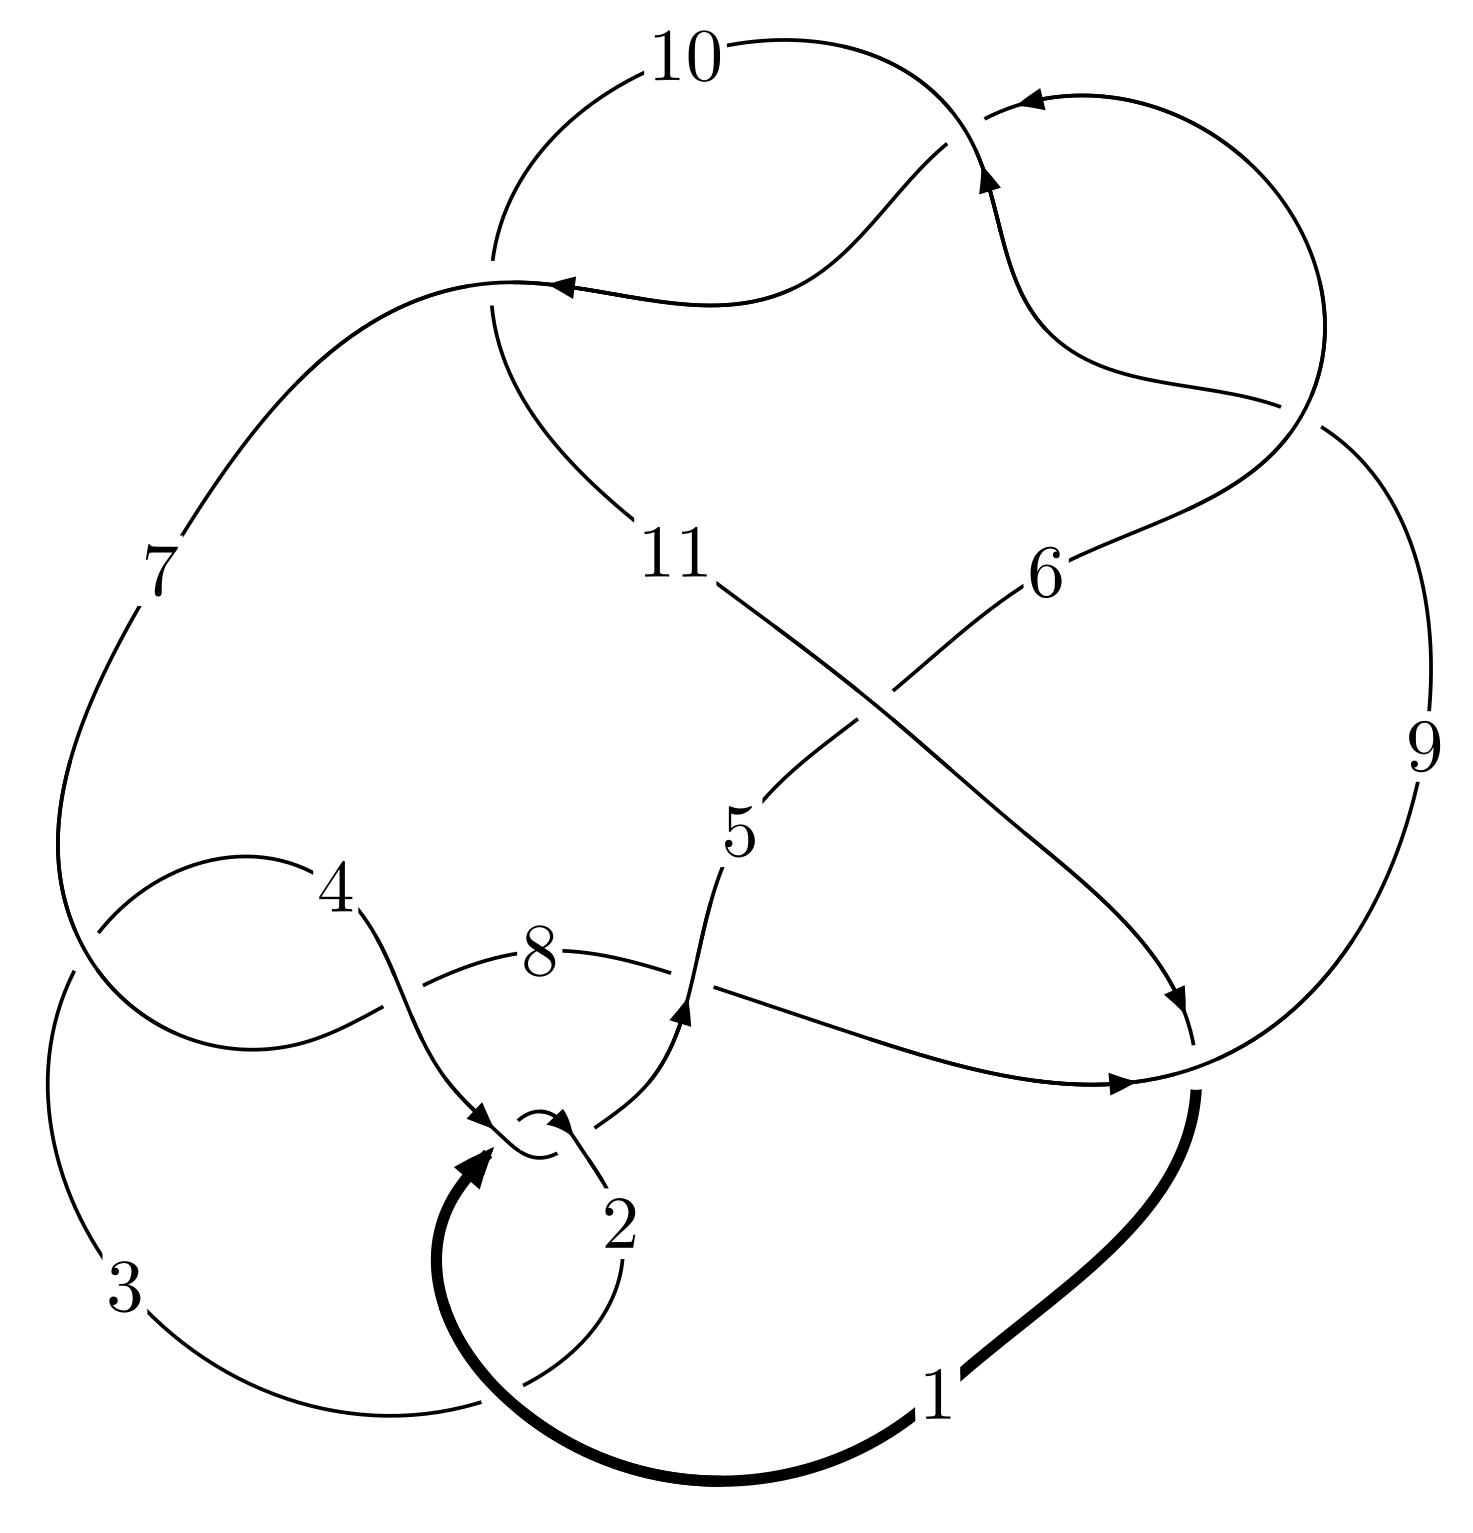
\includegraphics[width=112pt]{../../../GIT/diagram.site/Diagrams/png/675_11n_59.png}\\
\ \ \ A knot diagram\footnotemark}&
\allowdisplaybreaks
\textbf{Linearized knot diagam} \\
\cline{2-2}
 &
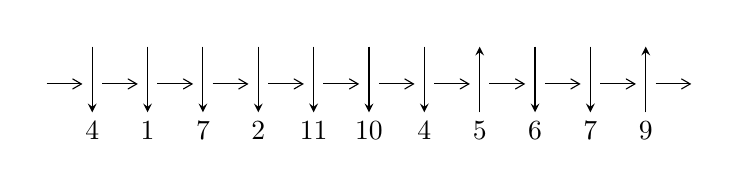
\begin{tikzpicture}[x=20pt, y=17pt]
	% nodes
	\node (C0) at (0, 0) {};
	\node (C1) at (1, 0) {};
	\node (C1U) at (1, +1) {};
	\node (C1D) at (1, -1) {4};

	\node (C2) at (2, 0) {};
	\node (C2U) at (2, +1) {};
	\node (C2D) at (2, -1) {1};

	\node (C3) at (3, 0) {};
	\node (C3U) at (3, +1) {};
	\node (C3D) at (3, -1) {7};

	\node (C4) at (4, 0) {};
	\node (C4U) at (4, +1) {};
	\node (C4D) at (4, -1) {2};

	\node (C5) at (5, 0) {};
	\node (C5U) at (5, +1) {};
	\node (C5D) at (5, -1) {11};

	\node (C6) at (6, 0) {};
	\node (C6U) at (6, +1) {};
	\node (C6D) at (6, -1) {10};

	\node (C7) at (7, 0) {};
	\node (C7U) at (7, +1) {};
	\node (C7D) at (7, -1) {4};

	\node (C8) at (8, 0) {};
	\node (C8U) at (8, +1) {};
	\node (C8D) at (8, -1) {5};

	\node (C9) at (9, 0) {};
	\node (C9U) at (9, +1) {};
	\node (C9D) at (9, -1) {6};

	\node (C10) at (10, 0) {};
	\node (C10U) at (10, +1) {};
	\node (C10D) at (10, -1) {7};

	\node (C11) at (11, 0) {};
	\node (C11U) at (11, +1) {};
	\node (C11D) at (11, -1) {9};
	\node (C12) at (12, 0) {};

	% arrows
	\draw[->,>={angle 60}]
	(C0) edge (C1) (C1) edge (C2) (C2) edge (C3) (C3) edge (C4) (C4) edge (C5) (C5) edge (C6) (C6) edge (C7) (C7) edge (C8) (C8) edge (C9) (C9) edge (C10) (C10) edge (C11) (C11) edge (C12) ;	\draw[->,>=stealth]
	(C1U) edge (C1D) (C2U) edge (C2D) (C3U) edge (C3D) (C4U) edge (C4D) (C5U) edge (C5D) (C6U) edge (C6D) (C7U) edge (C7D) (C8D) edge (C8U) (C9U) edge (C9D) (C10U) edge (C10D) (C11D) edge (C11U) ;
	\end{tikzpicture} \\
\hhline{~~} \\& 
\textbf{Solving Sequence} \\ \cline{2-2} 
 &
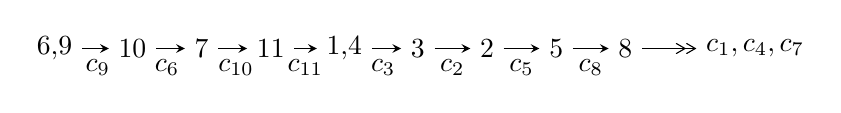
\begin{tikzpicture}[x=25pt, y=7pt]
	% node
	\node (A0) at (-1/8, 0) {6,9};
	\node (A1) at (1, 0) {10};
	\node (A2) at (2, 0) {7};
	\node (A3) at (3, 0) {11};
	\node (A4) at (65/16, 0) {1,4};
	\node (A5) at (41/8, 0) {3};
	\node (A6) at (49/8, 0) {2};
	\node (A7) at (57/8, 0) {5};
	\node (A8) at (65/8, 0) {8};
	\node (C1) at (1/2, -1) {$c_{9}$};
	\node (C2) at (3/2, -1) {$c_{6}$};
	\node (C3) at (5/2, -1) {$c_{10}$};
	\node (C4) at (7/2, -1) {$c_{11}$};
	\node (C5) at (37/8, -1) {$c_{3}$};
	\node (C6) at (45/8, -1) {$c_{2}$};
	\node (C7) at (53/8, -1) {$c_{5}$};
	\node (C8) at (61/8, -1) {$c_{8}$};
	\node (A9) at (10, 0) {$c_{1},c_{4},c_{7}$};

	% edge
	\draw[->,>=stealth]	
	(A0) edge (A1) (A1) edge (A2) (A2) edge (A3) (A3) edge (A4) (A4) edge (A5) (A5) edge (A6) (A6) edge (A7) (A7) edge (A8) ;
	\draw[->>,>={angle 60}]	
	(A8) edge (A9);
\end{tikzpicture} \\ 

\end{tabular} \\

\footnotetext{
The image of knot diagram is generated by the software ``\textbf{Draw programme}" developed by Andrew Bartholomew(\url{http://www.layer8.co.uk/maths/draw/index.htm\#Running-draw}), where we modified some parts for our purpose(\url{https://github.com/CATsTAILs/LinksPainter}).
}\phantom \\ \newline 
\centering \textbf{Ideals for irreducible components\footnotemark of $X_{\text{par}}$} 
 
\begin{align*}
I^u_{1}&=\langle 
u^{18}-8 u^{16}+25 u^{14}-36 u^{12}+19 u^{10}+4 u^8+2 u^7-2 u^6-6 u^5-4 u^4+4 u^3+u^2+b+2 u,\\
\phantom{I^u_{1}}&\phantom{= \langle  }- u^{29}- u^{28}+\cdots+a-1,\;u^{31}+2 u^{30}+\cdots+2 u+1\rangle \\
I^u_{2}&=\langle 
- u^4+2 u^2+b,\;- u^3+a+u+1,\;u^5- u^4-2 u^3+u^2+u+1\rangle \\
\\
\end{align*}
\raggedright * 2 irreducible components of $\dim_{\mathbb{C}}=0$, with total 36 representations.\\
\footnotetext{All coefficients of polynomials are rational numbers. But the coefficients are sometimes approximated in decimal forms when there is not enough margin.}
\newpage
\renewcommand{\arraystretch}{1}
\centering \section*{I. $I^u_{1}= \langle u^{18}-8 u^{16}+\cdots+b+2 u,\;- u^{29}- u^{28}+\cdots+a-1,\;u^{31}+2 u^{30}+\cdots+2 u+1 \rangle$}
\flushleft \textbf{(i) Arc colorings}\\
\begin{tabular}{m{7pt} m{180pt} m{7pt} m{180pt} }
\flushright $a_{6}=$&$\begin{pmatrix}0\\u\end{pmatrix}$ \\
\flushright $a_{9}=$&$\begin{pmatrix}1\\0\end{pmatrix}$ \\
\flushright $a_{10}=$&$\begin{pmatrix}1\\u^2\end{pmatrix}$ \\
\flushright $a_{7}=$&$\begin{pmatrix}- u\\- u^3+u\end{pmatrix}$ \\
\flushright $a_{11}=$&$\begin{pmatrix}- u^2+1\\- u^4+2 u^2\end{pmatrix}$ \\
\flushright $a_{1}=$&$\begin{pmatrix}- u^4+u^2+1\\- u^4+2 u^2\end{pmatrix}$ \\
\flushright $a_{4}=$&$\begin{pmatrix}u^{29}+u^{28}+\cdots+u+1\\- u^{18}+8 u^{16}+\cdots- u^2-2 u\end{pmatrix}$ \\
\flushright $a_{3}=$&$\begin{pmatrix}2 u^{30}+2 u^{29}+\cdots+2 u+2\\2 u^{30}+u^{29}+\cdots+u+2\end{pmatrix}$ \\
\flushright $a_{2}=$&$\begin{pmatrix}u^{30}+u^{29}+\cdots+2 u+2\\u^{30}-13 u^{28}+\cdots+7 u^3+1\end{pmatrix}$ \\
\flushright $a_{5}=$&$\begin{pmatrix}u^5-2 u^3+u\\u^7-3 u^5+2 u^3+u\end{pmatrix}$ \\
\flushright $a_{8}=$&$\begin{pmatrix}u^{12}-5 u^{10}+9 u^8-6 u^6+u^2+1\\u^{14}-6 u^{12}+13 u^{10}-10 u^8-2 u^6+4 u^4+u^2\end{pmatrix}$\\ \flushright $a_{8}=$&$\begin{pmatrix}u^{12}-5 u^{10}+9 u^8-6 u^6+u^2+1\\u^{14}-6 u^{12}+13 u^{10}-10 u^8-2 u^6+4 u^4+u^2\end{pmatrix}$\\&\end{tabular}
\flushleft \textbf{(ii) Obstruction class $= -1$}\\~\\
\flushleft \textbf{(iii) Cusp Shapes $= 2 u^{30}-26 u^{28}+5 u^{27}+147 u^{26}-59 u^{25}-460 u^{24}+296 u^{23}+817 u^{22}-799 u^{21}-658 u^{20}+1179 u^{19}-269 u^{18}-741 u^{17}+1010 u^{16}-254 u^{15}-570 u^{14}+536 u^{13}-222 u^{12}-2 u^{11}+186 u^{10}-168 u^9+98 u^8-68 u^7- u^6+41 u^5-40 u^4+35 u^3-19 u^2+5 u-6$}\\~\\
\newpage\renewcommand{\arraystretch}{1}
\flushleft \textbf{(iv) u-Polynomials at the component}\newline \\
\begin{tabular}{m{50pt}|m{274pt}}
Crossings & \hspace{64pt}u-Polynomials at each crossing \\
\hline $$\begin{aligned}c_{1},c_{4}\end{aligned}$$&$\begin{aligned}
&u^{31}-6 u^{30}+\cdots-4 u+1
\end{aligned}$\\
\hline $$\begin{aligned}c_{2}\end{aligned}$$&$\begin{aligned}
&u^{31}+8 u^{30}+\cdots+12 u+1
\end{aligned}$\\
\hline $$\begin{aligned}c_{3},c_{7}\end{aligned}$$&$\begin{aligned}
&u^{31}+u^{30}+\cdots+64 u+32
\end{aligned}$\\
\hline $$\begin{aligned}c_{5}\end{aligned}$$&$\begin{aligned}
&u^{31}-6 u^{30}+\cdots-18 u+5
\end{aligned}$\\
\hline $$\begin{aligned}c_{6},c_{9},c_{10}\end{aligned}$$&$\begin{aligned}
&u^{31}+2 u^{30}+\cdots+2 u+1
\end{aligned}$\\
\hline $$\begin{aligned}c_{8}\end{aligned}$$&$\begin{aligned}
&u^{31}-2 u^{30}+\cdots+2 u+1
\end{aligned}$\\
\hline $$\begin{aligned}c_{11}\end{aligned}$$&$\begin{aligned}
&u^{31}+8 u^{30}+\cdots+30 u+7
\end{aligned}$\\
\hline
\end{tabular}\\~\\
\newpage\renewcommand{\arraystretch}{1}
\flushleft \textbf{(v) Riley Polynomials at the component}\newline \\
\begin{tabular}{m{50pt}|m{274pt}}
Crossings & \hspace{64pt}Riley Polynomials at each crossing \\
\hline $$\begin{aligned}c_{1},c_{4}\end{aligned}$$&$\begin{aligned}
&y^{31}-8 y^{30}+\cdots+12 y-1
\end{aligned}$\\
\hline $$\begin{aligned}c_{2}\end{aligned}$$&$\begin{aligned}
&y^{31}+36 y^{30}+\cdots+48 y-1
\end{aligned}$\\
\hline $$\begin{aligned}c_{3},c_{7}\end{aligned}$$&$\begin{aligned}
&y^{31}+33 y^{30}+\cdots-10752 y-1024
\end{aligned}$\\
\hline $$\begin{aligned}c_{5}\end{aligned}$$&$\begin{aligned}
&y^{31}+4 y^{30}+\cdots+174 y-25
\end{aligned}$\\
\hline $$\begin{aligned}c_{6},c_{9},c_{10}\end{aligned}$$&$\begin{aligned}
&y^{31}-28 y^{30}+\cdots+2 y-1
\end{aligned}$\\
\hline $$\begin{aligned}c_{8}\end{aligned}$$&$\begin{aligned}
&y^{31}-36 y^{30}+\cdots+2 y-1
\end{aligned}$\\
\hline $$\begin{aligned}c_{11}\end{aligned}$$&$\begin{aligned}
&y^{31}+32 y^{29}+\cdots+1054 y-49
\end{aligned}$\\
\hline
\end{tabular}\\~\\
\newpage\flushleft \textbf{(vi) Complex Volumes and Cusp Shapes}
$$\begin{array}{c|c|c}  
\text{Solutions to }I^u_{1}& \I (\text{vol} + \sqrt{-1}CS) & \text{Cusp shape}\\
 \hline 
\begin{aligned}
u &= \phantom{-}0.953391 + 0.341205 I \\
a &= -0.060208 - 0.824217 I \\
b &= -0.154559 - 1.385810 I\end{aligned}
 & \phantom{-}5.55958 - 3.20800 I & -6.18542 + 3.44031 I \\ \hline\begin{aligned}
u &= \phantom{-}0.953391 - 0.341205 I \\
a &= -0.060208 + 0.824217 I \\
b &= -0.154559 + 1.385810 I\end{aligned}
 & \phantom{-}5.55958 + 3.20800 I & -6.18542 - 3.44031 I \\ \hline\begin{aligned}
u &= \phantom{-}0.825063 + 0.385979 I \\
a &= \phantom{-}0.618554 + 1.193580 I \\
b &= -0.63882 + 1.61785 I\end{aligned}
 & \phantom{-}5.21409 + 3.77786 I & -6.77733 - 1.30179 I \\ \hline\begin{aligned}
u &= \phantom{-}0.825063 - 0.385979 I \\
a &= \phantom{-}0.618554 - 1.193580 I \\
b &= -0.63882 - 1.61785 I\end{aligned}
 & \phantom{-}5.21409 - 3.77786 I & -6.77733 + 1.30179 I \\ \hline\begin{aligned}
u &= \phantom{-}0.256805 + 0.769307 I \\
a &= \phantom{-}1.018830 - 0.906649 I \\
b &= \phantom{-}0.90393 + 1.86214 I\end{aligned}
 & \phantom{-}7.07782 - 7.98216 I & -4.46644 + 5.97470 I \\ \hline\begin{aligned}
u &= \phantom{-}0.256805 - 0.769307 I \\
a &= \phantom{-}1.018830 + 0.906649 I \\
b &= \phantom{-}0.90393 - 1.86214 I\end{aligned}
 & \phantom{-}7.07782 + 7.98216 I & -4.46644 - 5.97470 I \\ \hline\begin{aligned}
u &= -1.191040 + 0.124902 I \\
a &= -0.150730 + 0.017487 I \\
b &= \phantom{-}0.447590 + 0.550052 I\end{aligned}
 & -1.84615 + 0.55694 I & -6.11373 + 0.01533 I \\ \hline\begin{aligned}
u &= -1.191040 - 0.124902 I \\
a &= -0.150730 - 0.017487 I \\
b &= \phantom{-}0.447590 - 0.550052 I\end{aligned}
 & -1.84615 - 0.55694 I & -6.11373 - 0.01533 I \\ \hline\begin{aligned}
u &= \phantom{-}0.195264 + 0.773377 I \\
a &= -1.255470 + 0.164780 I \\
b &= -0.177950 - 1.155760 I\end{aligned}
 & \phantom{-}7.92090 - 0.90622 I & -3.00591 + 1.13607 I \\ \hline\begin{aligned}
u &= \phantom{-}0.195264 - 0.773377 I \\
a &= -1.255470 - 0.164780 I \\
b &= -0.177950 + 1.155760 I\end{aligned}
 & \phantom{-}7.92090 + 0.90622 I & -3.00591 - 1.13607 I\\
 \hline 
 \end{array}$$\newpage$$\begin{array}{c|c|c}  
\text{Solutions to }I^u_{1}& \I (\text{vol} + \sqrt{-1}CS) & \text{Cusp shape}\\
 \hline 
\begin{aligned}
u &= -0.371835 + 0.568068 I \\
a &= \phantom{-}0.797944 - 0.031326 I \\
b &= -0.214074 - 0.837766 I\end{aligned}
 & -0.87857 + 1.75044 I & -3.85072 - 4.54648 I \\ \hline\begin{aligned}
u &= -0.371835 - 0.568068 I \\
a &= \phantom{-}0.797944 + 0.031326 I \\
b &= -0.214074 + 0.837766 I\end{aligned}
 & -0.87857 - 1.75044 I & -3.85072 + 4.54648 I \\ \hline\begin{aligned}
u &= \phantom{-}1.325090 + 0.154351 I \\
a &= -2.42287 + 0.53159 I \\
b &= -1.338960 - 0.362468 I\end{aligned}
 & -5.25829 - 1.15681 I & -12.57201 + 1.48822 I \\ \hline\begin{aligned}
u &= \phantom{-}1.325090 - 0.154351 I \\
a &= -2.42287 - 0.53159 I \\
b &= -1.338960 + 0.362468 I\end{aligned}
 & -5.25829 + 1.15681 I & -12.57201 - 1.48822 I \\ \hline\begin{aligned}
u &= -0.156640 + 0.637516 I \\
a &= -0.041090 - 1.349110 I \\
b &= -0.896955 + 0.568672 I\end{aligned}
 & \phantom{-}1.00966 + 2.22196 I & -3.40092 - 5.38737 I \\ \hline\begin{aligned}
u &= -0.156640 - 0.637516 I \\
a &= -0.041090 + 1.349110 I \\
b &= -0.896955 - 0.568672 I\end{aligned}
 & \phantom{-}1.00966 - 2.22196 I & -3.40092 + 5.38737 I \\ \hline\begin{aligned}
u &= -1.351700 + 0.206762 I \\
a &= \phantom{-}0.051503 - 0.972430 I \\
b &= -0.62993 - 1.46088 I\end{aligned}
 & -6.05722 + 3.45238 I & -10.37888 - 2.19312 I \\ \hline\begin{aligned}
u &= -1.351700 - 0.206762 I \\
a &= \phantom{-}0.051503 + 0.972430 I \\
b &= -0.62993 + 1.46088 I\end{aligned}
 & -6.05722 - 3.45238 I & -10.37888 + 2.19312 I \\ \hline\begin{aligned}
u &= \phantom{-}1.355400 + 0.255032 I \\
a &= \phantom{-}1.82855 - 0.84093 I \\
b &= \phantom{-}1.180600 + 0.666054 I\end{aligned}
 & -3.77819 - 5.48065 I & -9.45984 + 5.94075 I \\ \hline\begin{aligned}
u &= \phantom{-}1.355400 - 0.255032 I \\
a &= \phantom{-}1.82855 + 0.84093 I \\
b &= \phantom{-}1.180600 - 0.666054 I\end{aligned}
 & -3.77819 + 5.48065 I & -9.45984 - 5.94075 I\\
 \hline 
 \end{array}$$\newpage$$\begin{array}{c|c|c}  
\text{Solutions to }I^u_{1}& \I (\text{vol} + \sqrt{-1}CS) & \text{Cusp shape}\\
 \hline 
\begin{aligned}
u &= -1.374710 + 0.318270 I \\
a &= \phantom{-}1.72875 - 0.73774 I \\
b &= \phantom{-}0.359105 - 0.934571 I\end{aligned}
 & \phantom{-}2.95558 + 4.85038 I & -7.33363 - 2.61184 I \\ \hline\begin{aligned}
u &= -1.374710 - 0.318270 I \\
a &= \phantom{-}1.72875 + 0.73774 I \\
b &= \phantom{-}0.359105 + 0.934571 I\end{aligned}
 & \phantom{-}2.95558 - 4.85038 I & -7.33363 + 2.61184 I \\ \hline\begin{aligned}
u &= -1.40893 + 0.31052 I \\
a &= -2.64694 + 0.69829 I \\
b &= -1.12415 + 1.93346 I\end{aligned}
 & \phantom{-}1.77560 + 11.89500 I & -8.90588 - 6.87931 I \\ \hline\begin{aligned}
u &= -1.40893 - 0.31052 I \\
a &= -2.64694 - 0.69829 I \\
b &= -1.12415 - 1.93346 I\end{aligned}
 & \phantom{-}1.77560 - 11.89500 I & -8.90588 + 6.87931 I \\ \hline\begin{aligned}
u &= -1.45164 + 0.04136 I \\
a &= \phantom{-}0.77948 + 1.85121 I \\
b &= \phantom{-}0.915385 + 0.997789 I\end{aligned}
 & -1.95006 - 2.95334 I & -10.65956 + 2.73175 I \\ \hline\begin{aligned}
u &= -1.45164 - 0.04136 I \\
a &= \phantom{-}0.77948 - 1.85121 I \\
b &= \phantom{-}0.915385 - 0.997789 I\end{aligned}
 & -1.95006 + 2.95334 I & -10.65956 - 2.73175 I \\ \hline\begin{aligned}
u &= \phantom{-}1.43633 + 0.21708 I \\
a &= -0.458519 - 1.234670 I \\
b &= \phantom{-}0.376409 - 1.104670 I\end{aligned}
 & -6.67621 - 4.65354 I & -6.91647 + 4.60285 I \\ \hline\begin{aligned}
u &= \phantom{-}1.43633 - 0.21708 I \\
a &= -0.458519 + 1.234670 I \\
b &= \phantom{-}0.376409 + 1.104670 I\end{aligned}
 & -6.67621 + 4.65354 I & -6.91647 - 4.60285 I \\ \hline\begin{aligned}
u &= \phantom{-}0.127284 + 0.484686 I \\
a &= \phantom{-}0.09092 + 1.50930 I \\
b &= \phantom{-}0.622522 - 0.861672 I\end{aligned}
 & -1.33374 - 0.83076 I & -4.07951 - 0.75098 I \\ \hline\begin{aligned}
u &= \phantom{-}0.127284 - 0.484686 I \\
a &= \phantom{-}0.09092 - 1.50930 I \\
b &= \phantom{-}0.622522 + 0.861672 I\end{aligned}
 & -1.33374 + 0.83076 I & -4.07951 + 0.75098 I\\
 \hline 
 \end{array}$$\newpage$$\begin{array}{c|c|c}  
\text{Solutions to }I^u_{1}& \I (\text{vol} + \sqrt{-1}CS) & \text{Cusp shape}\\
 \hline 
\begin{aligned}
u &= -0.336229\phantom{ +0.000000I} \\
a &= \phantom{-}1.24262\phantom{ +0.000000I} \\
b &= \phantom{-}0.739715\phantom{ +0.000000I}\end{aligned}
 & -0.889878\phantom{ +0.000000I} & -11.7880\phantom{ +0.000000I}\\
 \hline 
 \end{array}$$\newpage\newpage\renewcommand{\arraystretch}{1}
\centering \section*{II. $I^u_{2}= \langle - u^4+2 u^2+b,\;- u^3+a+u+1,\;u^5- u^4-2 u^3+u^2+u+1 \rangle$}
\flushleft \textbf{(i) Arc colorings}\\
\begin{tabular}{m{7pt} m{180pt} m{7pt} m{180pt} }
\flushright $a_{6}=$&$\begin{pmatrix}0\\u\end{pmatrix}$ \\
\flushright $a_{9}=$&$\begin{pmatrix}1\\0\end{pmatrix}$ \\
\flushright $a_{10}=$&$\begin{pmatrix}1\\u^2\end{pmatrix}$ \\
\flushright $a_{7}=$&$\begin{pmatrix}- u\\- u^3+u\end{pmatrix}$ \\
\flushright $a_{11}=$&$\begin{pmatrix}- u^2+1\\- u^4+2 u^2\end{pmatrix}$ \\
\flushright $a_{1}=$&$\begin{pmatrix}- u^4+u^2+1\\- u^4+2 u^2\end{pmatrix}$ \\
\flushright $a_{4}=$&$\begin{pmatrix}u^3- u-1\\u^4-2 u^2\end{pmatrix}$ \\
\flushright $a_{3}=$&$\begin{pmatrix}u^3- u-1\\u^4-2 u^2\end{pmatrix}$ \\
\flushright $a_{2}=$&$\begin{pmatrix}- u^4+u^3+u^2- u\\0\end{pmatrix}$ \\
\flushright $a_{5}=$&$\begin{pmatrix}u^4- u^2-1\\u^4-2 u^2\end{pmatrix}$ \\
\flushright $a_{8}=$&$\begin{pmatrix}- u\\- u^3+u\end{pmatrix}$\\ \flushright $a_{8}=$&$\begin{pmatrix}- u\\- u^3+u\end{pmatrix}$\\&\end{tabular}
\flushleft \textbf{(ii) Obstruction class $= 1$}\\~\\
\flushleft \textbf{(iii) Cusp Shapes $= 3 u^3+u^2-8 u-15$}\\~\\
\newpage\renewcommand{\arraystretch}{1}
\flushleft \textbf{(iv) u-Polynomials at the component}\newline \\
\begin{tabular}{m{50pt}|m{274pt}}
Crossings & \hspace{64pt}u-Polynomials at each crossing \\
\hline $$\begin{aligned}c_{1}\end{aligned}$$&$\begin{aligned}
&(u-1)^5
\end{aligned}$\\
\hline $$\begin{aligned}c_{2},c_{4}\end{aligned}$$&$\begin{aligned}
&(u+1)^5
\end{aligned}$\\
\hline $$\begin{aligned}c_{3},c_{7}\end{aligned}$$&$\begin{aligned}
&u^5
\end{aligned}$\\
\hline $$\begin{aligned}c_{5}\end{aligned}$$&$\begin{aligned}
&u^5-3 u^4+4 u^3- u^2- u+1
\end{aligned}$\\
\hline $$\begin{aligned}c_{6}\end{aligned}$$&$\begin{aligned}
&u^5+u^4-2 u^3- u^2+u-1
\end{aligned}$\\
\hline $$\begin{aligned}c_{8},c_{11}\end{aligned}$$&$\begin{aligned}
&u^5+u^4+2 u^3+u^2+u+1
\end{aligned}$\\
\hline $$\begin{aligned}c_{9},c_{10}\end{aligned}$$&$\begin{aligned}
&u^5- u^4-2 u^3+u^2+u+1
\end{aligned}$\\
\hline
\end{tabular}\\~\\
\newpage\renewcommand{\arraystretch}{1}
\flushleft \textbf{(v) Riley Polynomials at the component}\newline \\
\begin{tabular}{m{50pt}|m{274pt}}
Crossings & \hspace{64pt}Riley Polynomials at each crossing \\
\hline $$\begin{aligned}c_{1},c_{2},c_{4}\end{aligned}$$&$\begin{aligned}
&(y-1)^5
\end{aligned}$\\
\hline $$\begin{aligned}c_{3},c_{7}\end{aligned}$$&$\begin{aligned}
&y^5
\end{aligned}$\\
\hline $$\begin{aligned}c_{5}\end{aligned}$$&$\begin{aligned}
&y^5- y^4+8 y^3-3 y^2+3 y-1
\end{aligned}$\\
\hline $$\begin{aligned}c_{6},c_{9},c_{10}\end{aligned}$$&$\begin{aligned}
&y^5-5 y^4+8 y^3-3 y^2- y-1
\end{aligned}$\\
\hline $$\begin{aligned}c_{8},c_{11}\end{aligned}$$&$\begin{aligned}
&y^5+3 y^4+4 y^3+y^2- y-1
\end{aligned}$\\
\hline
\end{tabular}\\~\\
\newpage\flushleft \textbf{(vi) Complex Volumes and Cusp Shapes}
$$\begin{array}{c|c|c}  
\text{Solutions to }I^u_{2}& \I (\text{vol} + \sqrt{-1}CS) & \text{Cusp shape}\\
 \hline 
\begin{aligned}
u &= -1.21774\phantom{ +0.000000I} \\
a &= -1.58802\phantom{ +0.000000I} \\
b &= -0.766826\phantom{ +0.000000I}\end{aligned}
 & -4.04602\phantom{ +0.000000I} & -9.19250\phantom{ +0.000000I} \\ \hline\begin{aligned}
u &= -0.309916 + 0.549911 I \\
a &= -0.438694 - 0.557752 I \\
b &= \phantom{-}0.339110 + 0.822375 I\end{aligned}
 & -1.97403 + 1.53058 I & -11.97286 - 4.76366 I \\ \hline\begin{aligned}
u &= -0.309916 - 0.549911 I \\
a &= -0.438694 + 0.557752 I \\
b &= \phantom{-}0.339110 - 0.822375 I\end{aligned}
 & -1.97403 - 1.53058 I & -11.97286 + 4.76366 I \\ \hline\begin{aligned}
u &= \phantom{-}1.41878 + 0.21917 I \\
a &= \phantom{-}0.232705 + 1.093810 I \\
b &= -0.455697 + 1.200150 I\end{aligned}
 & -7.51750 - 4.40083 I & -16.4309 + 2.8075 I \\ \hline\begin{aligned}
u &= \phantom{-}1.41878 - 0.21917 I \\
a &= \phantom{-}0.232705 - 1.093810 I \\
b &= -0.455697 - 1.200150 I\end{aligned}
 & -7.51750 + 4.40083 I & -16.4309 - 2.8075 I\\
 \hline 
 \end{array}$$\newpage
\newpage\renewcommand{\arraystretch}{1}
\centering \section*{ III. u-Polynomials}
\begin{tabular}{m{50pt}|m{274pt}}
Crossings & \hspace{64pt}u-Polynomials at each crossing \\
\hline $$\begin{aligned}c_{1}\end{aligned}$$&$\begin{aligned}
&((u-1)^5)(u^{31}-6 u^{30}+\cdots-4 u+1)
\end{aligned}$\\
\hline $$\begin{aligned}c_{2}\end{aligned}$$&$\begin{aligned}
&((u+1)^5)(u^{31}+8 u^{30}+\cdots+12 u+1)
\end{aligned}$\\
\hline $$\begin{aligned}c_{3},c_{7}\end{aligned}$$&$\begin{aligned}
&u^5(u^{31}+u^{30}+\cdots+64 u+32)
\end{aligned}$\\
\hline $$\begin{aligned}c_{4}\end{aligned}$$&$\begin{aligned}
&((u+1)^5)(u^{31}-6 u^{30}+\cdots-4 u+1)
\end{aligned}$\\
\hline $$\begin{aligned}c_{5}\end{aligned}$$&$\begin{aligned}
&(u^5-3 u^4+4 u^3- u^2- u+1)(u^{31}-6 u^{30}+\cdots-18 u+5)
\end{aligned}$\\
\hline $$\begin{aligned}c_{6}\end{aligned}$$&$\begin{aligned}
&(u^5+u^4-2 u^3- u^2+u-1)(u^{31}+2 u^{30}+\cdots+2 u+1)
\end{aligned}$\\
\hline $$\begin{aligned}c_{8}\end{aligned}$$&$\begin{aligned}
&(u^5+u^4+2 u^3+u^2+u+1)(u^{31}-2 u^{30}+\cdots+2 u+1)
\end{aligned}$\\
\hline $$\begin{aligned}c_{9},c_{10}\end{aligned}$$&$\begin{aligned}
&(u^5- u^4-2 u^3+u^2+u+1)(u^{31}+2 u^{30}+\cdots+2 u+1)
\end{aligned}$\\
\hline $$\begin{aligned}c_{11}\end{aligned}$$&$\begin{aligned}
&(u^5+u^4+2 u^3+u^2+u+1)(u^{31}+8 u^{30}+\cdots+30 u+7)
\end{aligned}$\\
\hline
\end{tabular}\newpage\renewcommand{\arraystretch}{1}
\centering \section*{ IV. Riley Polynomials}
\begin{tabular}{m{50pt}|m{274pt}}
Crossings & \hspace{64pt}Riley Polynomials at each crossing \\
\hline $$\begin{aligned}c_{1},c_{4}\end{aligned}$$&$\begin{aligned}
&((y-1)^5)(y^{31}-8 y^{30}+\cdots+12 y-1)
\end{aligned}$\\
\hline $$\begin{aligned}c_{2}\end{aligned}$$&$\begin{aligned}
&((y-1)^5)(y^{31}+36 y^{30}+\cdots+48 y-1)
\end{aligned}$\\
\hline $$\begin{aligned}c_{3},c_{7}\end{aligned}$$&$\begin{aligned}
&y^5(y^{31}+33 y^{30}+\cdots-10752 y-1024)
\end{aligned}$\\
\hline $$\begin{aligned}c_{5}\end{aligned}$$&$\begin{aligned}
&(y^5- y^4+8 y^3-3 y^2+3 y-1)(y^{31}+4 y^{30}+\cdots+174 y-25)
\end{aligned}$\\
\hline $$\begin{aligned}c_{6},c_{9},c_{10}\end{aligned}$$&$\begin{aligned}
&(y^5-5 y^4+8 y^3-3 y^2- y-1)(y^{31}-28 y^{30}+\cdots+2 y-1)
\end{aligned}$\\
\hline $$\begin{aligned}c_{8}\end{aligned}$$&$\begin{aligned}
&(y^5+3 y^4+4 y^3+y^2- y-1)(y^{31}-36 y^{30}+\cdots+2 y-1)
\end{aligned}$\\
\hline $$\begin{aligned}c_{11}\end{aligned}$$&$\begin{aligned}
&(y^5+3 y^4+4 y^3+y^2- y-1)(y^{31}+32 y^{29}+\cdots+1054 y-49)
\end{aligned}$\\
\hline
\end{tabular}
\vskip 2pc
\end{document}